\documentclass[12pt,a4paper,oneside]{report}

% ---------------- Layout & Paket Dasar ----------------
\usepackage[a4paper, top=4cm, left=3cm, right=3cm, bottom=3cm]{geometry}
\usepackage{setspace}      % untuk kontrol spasi
\usepackage{titlesec}      % untuk atur ukuran heading
\usepackage{graphicx}
\usepackage{listings}      % untuk "Daftar Tampilan" (kode/program)
\usepackage{caption}
\usepackage{fontspec}
\usepackage[backend=biber,style=ieee,sorting=nyt]{biblatex}
\usepackage{pdflscape}   % halaman landscape (auto-rotate di PDF)
\usepackage{longtable}   % tabel multi-halaman
\usepackage{booktabs}    % garis tabel yang rapi
\usepackage{multirow}    % opsional, jika ingin menggabung baris
\usepackage{array}       % untuk p{width} yang stabil
\usepackage{float}
\usepackage{plantuml} % butuh compile dengan -shell-escape
\usepackage{amsmath}
\usepackage{microtype}

\emergencystretch=2em
\addbibresource{proposal_desertasi_version_1.bib}
\setmainfont{Times New Roman} % ganti ke "TeX Gyre Termes" bila TNR tidak tersedia

% ---------------- Ukuran heading -----------------------
% Judul Bab = 14pt bold, center, dengan label BAB + angka Romawi
\titleformat{\chapter}[display]
    {\centering\bfseries\fontsize{14pt}{16pt}\selectfont}
    {BAB \Roman{chapter}}
    {0pt}
    {\vspace{1ex}}
    [\vspace{1ex}]

% Atur jarak judul bab: margin atas tetap 4cm
\titlespacing*{\chapter}{0pt}{0pt}{0.5cm}

% Subjudul (section, subsection) = 13pt bold
\titleformat{\section}
    {\bfseries\fontsize{13pt}{15pt}\selectfont}
    {\thesection}{1em}{}
\titlespacing*{\section}{0pt}{1.0\baselineskip}{1\baselineskip}

\titleformat{\subsection}
    {\bfseries\fontsize{13pt}{15pt}\selectfont}
    {\thesubsection}{1em}{}

% ---------------- Bibliografi (spasi 1) ----------------
\AtBeginBibliography{\singlespacing} % daftar pustaka spasi 1

\begin{document}
    % ===================== HALAMAN JUDUL (spasi 1) =====================
    \begin{titlepage}
        \thispagestyle{empty} % No page number
        \begin{center}
            \Large{\textbf{USULAN PENELITIAN DISERTASI}}\\[0.5cm]
            \Large{\textbf{DATA ALIGNMENT BERBASIS PROBABILISTIC ENTITY RESOLUTION DAN DETEKSI ANOMALI KEPATUHAN YANG TERINTEGRASI DENGAN RETRIEVAL AUGMENTED GENERATION}}\\[0.5cm]
            \Large{(DATA ALIGNMENT BASED ON PROBABILISTIC ENTITY RESOLUTION AND COMPLIANCE ANOMALY DETECTION INTEGRATED WITH RETRIEVAL AUGMENTED GENERATION)}\\[0.5cm]

            \large{\textbf{disusun dan diajukan oleh}}\\
            \large{\textbf{Benny Leonard Enrico Panggabean}}\\
            \large{\textbf{D063251008}}\\[2cm]

            
\includegraphics[width=5cm]{Logo-Resmi-Unhas-1.png}\\[1.5cm] % Replace with actual logo file

            \large{\textbf{PROGRAM STUDI DOKTOR TEKNIK INFORMATIKA}}\\
            \large{\textbf{FAKULTAS TEKNIK}}\\
            \large{\textbf{UNIVERSITAS HASANUDDIN}}\\
            \large{\textbf{MAKASSAR}}\\
            \large{\textbf{2025}}\\
        \end{center}
    \end{titlepage}
    % ===================== HALAMAN BAB 1 (spasi 1.5) =====================
    \onehalfspacing
    
    \chapter{PENDAHULUAN}
        \thispagestyle{empty} % No page number
        \section{Latar Belakang}
            % start paragraf
            Pendidikan tinggi di Indonesia memegang peran sentral dalam pembangunan sumber daya manusia unggul, pengembangan ilmu pengetahuan dan teknologi, serta kontribusi terhadap kesejahteraan masyarakat melalui tridharma perguruan tinggi.
            Untuk menjamin mutu penyelenggaraan tridharma tersebut, pemerintah melalui Kementerian Pendidikan, Kebudayaan, Riset, dan Teknologi menetapkan Permendikbudristek Nomor 39 Tahun 2025 tentang Penjaminan Mutu Pendidikan Tinggi. Peraturan ini memperbarui ketentuan sebelumnya pada Permendikbudristek Nomor 53 Tahun 2023, dengan penekanan pada penguatan integrasi sistem mutu dengan Pangkalan Data Pendidikan Tinggi (PDDikti) dan peningkatan relevansi standar mutu pendidikan tinggi terhadap perkembangan global.
            Permendikbudristek Nomor 39 Tahun 2025 menegaskan bahwa penjaminan mutu pendidikan tinggi dilaksanakan secara sistemik, terencana, berkelanjutan, dan menyeluruh, meliputi standar pendidikan, penelitian, dan pengabdian kepada masyarakat yang dirumuskan dalam Standar Nasional Pendidikan Tinggi (SN-Dikti). Perguruan tinggi wajib melaksanakan Sistem Penjaminan Mutu Internal (SPMI) dan mengikuti Sistem Penjaminan Mutu Eksternal (SPME) melalui mekanisme akreditasi. PDDikti menjadi rujukan utama dalam memantau kepatuhan terhadap SN-Dikti, sekaligus menjadi instrumen strategis untuk penilaian kinerja, akreditasi, dan pengambilan kebijakan.
            Kualitas data yang dilaporkan ke PDDikti sangat menentukan akuntabilitas dan kredibilitas perguruan tinggi.
            Data yang tidak sinkron, tidak akurat, atau tidak sesuai regulasi dapat berdampak langsung pada penurunan status akreditasi,
            berkurangnya kepercayaan publik, hingga menimbulkan kerugian bagi mahasiswa. Faktanya,
            dalam praktik pelaporan akademik melalui Sistem Informasi Akademik (SIAKAD) internal dan FEEDER PDDikti, sering ditemukan berbagai masalah:
            \begin{enumerate}
                \item Ketidaksinkronan data, misalnya perbedaan penulisan nama mahasiswa/dosen atau perbedaan jumlah SKS.
                \item Perbedaan struktur data antara SIAKAD dan FEEDER
                \item Anomali kepatuhan, seperti dosen tercatat mengajar lebih dari 16 SKS per semester, mahasiswa aktif melebihi daya tampung resmi, atau mahasiswa dengan masa studi melebihi ketentuan tanpa status jelas.
            \end{enumerate}
            Kondisi ini menjadi tantangan besar, terutama di daerah dengan jumlah perguruan tinggi yang signifikan. Berdasarkan data Pangkalan Data Perguruan Tinggi pada tahun~2025,
            terdapat 367~perguruan tinggi (negeri dan swasta) di Provinsi Sulawesi Selatan. Angka tersebut mencerminkan keragaman kapasitas dan sumber daya institusi,
            yang seluruhnya wajib melaporkan data akademik secara akurat dan konsisten ke PDDikti.
            Kompleksitas ini mempertegas pentingnya solusi teknologi untuk memastikan keselarasan data dan kepatuhan regulasi.
            Perkembangan teknologi kecerdasan buatan (AI) memberikan peluang untuk mengatasi permasalahan ini.
            Probabilistic Entity Resolution (ER) memungkinkan penyelarasan data antar sistem dengan memperhitungkan perbedaan format, struktur, maupun variasi penulisan.
            Dengan pendekatan probabilistik, sistem dapat menghitung tingkat keyakinan (confidence score) apakah dua entitas dari SIAKAD dan FEEDER merepresentasikan individu atau unit yang sama.
            Setelah data selaras, deteksi anomali kepatuhan menjadi tahap krusial berikutnya. Pendekatan hybrid yang menggabungkan aturan regulasi (rule-based) dan machine learning (misalnya Isolation Forest, Local Outlier Factor, atau Autoencoder) dapat mendeteksi ketidakwajaran dalam data.
            Contohnya, sistem bisa menandai dosen dengan beban SKS berlebih, mahasiswa yang ganda, atau prodi yang melaporkan daya tampung tidak konsisten.
            Hasil dari entity resolution dan anomaly detection ini kemudian dapat diintegrasikan ke dalam Retrieval-Augmented Generation (RAG). Dengan mekanisme ini,
            pimpinan program studi dapat mengajukan pertanyaan, dan sistem akan memberikan jawaban berbukti yang menggabungkan regulasi resmi (Permendikbudristek No. 39 Tahun 2025) dengan data ter-align dari SIAKAD–FEEDER serta temuan anomali kepatuhan.
            Jawaban dilengkapi dengan sitasi dan confidence score, sehingga dapat dipertanggungjawabkan.
            Dengan demikian, penelitian mengenai “Data alignment berbasis probabilistic entity resolution dan deteksi anomali kepatuhan yang terintegrasi RAG” memiliki urgensi tinggi.
            Penelitian ini tidak hanya menjawab masalah teknis sinkronisasi dan validasi data akademik, tetapi juga mendukung implementasi regulasi terbaru, yaitu Permendikbudristek Nomor 39 Tahun 2025, sekaligus memperkuat sistem penjaminan mutu pendidikan tinggi di Indonesia.
            Melalui kontribusi akademis dan praktis, penelitian ini diharapkan dapat meningkatkan kualitas tata kelola data, mendukung akreditasi, dan memperkuat kepercayaan publik terhadap perguruan tinggi, khususnya di Provinsi Sulawesi Selatan.
        \section{Rumusan Masalah}
            % start paragraf
            Berdasarkan latar belakang yang telah dipaparkan, maka rumusan masalah penelitian ini dapat dirumuskan sebagai berikut:
            \begin{enumerate}
                \item Menganalisis perbedaan struktur, format, dan kualitas data antara sistem SIAKAD internal perguruan tinggi dengan FEEDER PDDikti, serta dampaknya terhadap mutu pelaporan akademik dan kepatuhan regulasi pendidikan tinggi.
                
                \item Mengevaluasi efektivitas metode \textit{probabilistic entity resolution} dalam menyelaraskan data antar sistem (\textit{data alignment}),
                    khususnya untuk entitas mahasiswa, dosen, program studi, dan mata kuliah dengan mempertimbangkan konteks data akademik Indonesia.
                \item Merancang model deteksi anomali kepatuhan (compliance anomaly detection) berbasis pendekatan hybrid (rule-based dan machine learning) untuk mengidentifikasi pelanggaran terhadap standar regulasi, seperti beban SKS dosen, daya tampung mahasiswa, dan masa studi.
                \item Mengintegrasikan hasil entity resolution dan anomaly detection dengan pendekatan Retrieval-Augmented Generation (RAG) agar dapat menghasilkan jawaban tanya-jawab akademik yang akurat, berbukti, dan selaras dengan regulasi yang berlaku.
                \item Mengukur dan membandingkan performa sistem yang diusulkan dengan baseline eksisting, menggunakan metrik evaluasi seperti precision, recall, F1-score (entity resolution), AUC dan anomaly detection, serta citation precision dan faithfulness (RAG).
                \item Mendesain kerangka evaluasi end-to-end yang menggabungkan aspek teknis (akurasi, performa), aspek regulatif (kepatuhan terhadap Permendikbudristek Nomor 39 Tahun 2025), serta aspek praktis (kebermanfaatan bagi pimpinan program studi dalam pengambilan keputusan).
            \end{enumerate}
        \section{Tujuan Penelitian}
            % start paragraf
            Adapun tujuan dari penelitian ini adalah sebagai berikut:
            \begin{enumerate}
                \item Menganalisis karakteristik ketidaksinkronan data antara SIAKAD dan FEEDER PDDikti, termasuk variasi struktur, format, serta standar penulisan, guna memahami sumber masalah dalam pelaporan akademik.
                \item Mengevaluasi penerapan metode probabilistic entity resolution untuk penyelarasan data akademik, dengan membandingkan kinerjanya terhadap pendekatan rule-based tradisional.
                \item Merancang model deteksi anomali kepatuhan berbasis pendekatan hybrid (rule-based dan machine learning) yang mampu mengidentifikasi dan mengklasifikasikan ketidaksesuaian dengan regulasi pendidikan tinggi.
                \item Mengintegrasikan hasil entity resolution dan anomaly detection ke dalam sistem Retrieval-Augmented Generation (RAG), sehingga sistem dapat memberikan jawaban berbukti yang akurat, konsisten, dan sesuai regulasi.
                \item Mengukur dan membandingkan efektivitas sistem yang diusulkan dengan baseline eksisting menggunakan metrik kuantitatif (precision, recall, F1-score, AUC, citation precision, faithfulness) dan evaluasi kualitatif (user study dengan pimpinan program studi).
                \item Mengembangkan kerangka evaluasi end-to-end untuk sistem audit kepatuhan akademik berbasis Kecerdasan Buatan yang selaras dengan regulasi terbaru, yakni Permendikbudristek Nomor 39 Tahun 2025, serta relevan untuk peningkatan mutu tata kelola pendidikan tinggi di Indonesia.
            \end{enumerate}
        \section{Batasan Masalah}
            Agar penelitian ini terarah dan fokus, maka ruang lingkup penelitian dibatasi pada hal-hal berikut:
            % start paragraf
            \begin{enumerate}
                \item Objek Data, Data bersumber dari Sistem Informasi Akademik (SIAKAD) internal perguruan tinggi dan FEEDER PDDikti sebagai kanal pelaporan resmi.
                \item Cakupan Regulasi, Regulasi yang dijadikan rujukan utama adalah Permendikbudristek Nomor 39 Tahun 2025 tentang Penjaminan Mutu Pendidikan Tinggi, serta aturan terkait standar beban dosen, masa studi, daya tampung, dan standar akreditasi.
                    Peraturan sebelumnya seperti Permendikbudristek Nomor 53 Tahun 2023 diposisikan sebagai referensi historis.
                \item Metode Teknis
                    \begin{itemize}
                        \item Entity Resolution difokuskan pada pendekatan probabilistik yang dapat dipadukan dengan pembelajaran mesin (machine learning) dan representasi berbasis embedding.
                        \item Deteksi anomali kepatuhan difokuskan pada metode hybrid: aturan regulasi (rule-based) dan algoritma deteksi outlier (misalnya Isolation Forest, LOF, Autoencoder).
                        \item RAG (Retrieval-Augmented Generation) difokuskan pada integrasi dengan data hasil alignment dan anomaly detection, bukan pada pengembangan arsitektur LLM baru.
                    \end{itemize}
                \item Ruang Evaluasi
                    \begin{itemize}
                        \item Evaluasi sistem dilakukan melalui metrik kuantitatif (precision, recall, F1-score, AUC, faithfulness) dan studi pengguna (user study) pada level pimpinan program studi.
                        \item Penelitian tidak mencakup implementasi skala nasional di semua perguruan tinggi, melainkan studi kasus yang dapat digeneralisasikan.
                    \end{itemize}
            \end{enumerate}
        \section{Manfaat Penelitian}
            % start paragraf
            Penelitian ini diharapkan memberikan manfaat pada tiga level: teoritis, praktis, dan kebijakan.
            \begin{enumerate}
                \item Manfaat Teoritis
                    \begin{itemize}
                        \item Memberikan kontribusi pada pengembangan ilmu di bidang data integration, anomaly detection, dan retrieval-augmented generation.
                        \item Menghasilkan kerangka metodologis baru untuk confidence-aware RAG yang menggabungkan probabilistic entity resolution dan anomaly detection.
                    \end{itemize}
                \item Manfaat Praktis
                    \begin{itemize}
                        \item Menyediakan prototipe sistem audit kepatuhan akademik berbasis AI yang dapat digunakan oleh perguruan tinggi.
                        \item Membantu pimpinan program studi dalam mengambil keputusan cepat, akurat, dan berbukti, terutama terkait kepatuhan regulasi dan pelaporan data.
                        \item Menurunkan beban kerja manual staf akademik dalam sinkronisasi data SIAKAD–FEEDER.
                    \end{itemize}
                \item Manfaat Kebijakan
                    \begin{itemize}
                        \item Mendukung implementasi Permendikbudristek Nomor 39 Tahun 2025 melalui penyediaan mekanisme audit kepatuhan berbasis data dan Kecerdasan Buatan.
                        \item Menjadi masukan bagi pemerintah dan lembaga akreditasi dalam menyusun kebijakan penjaminan mutu berbasis data yang lebih adaptif dan transparan.
                        \item Memberikan landasan bagi pengembangan standar evaluasi nasional dalam integritas data akademik dan pelaporan PDDikti.
                    \end{itemize}
            \end{enumerate}
    % ===================== HALAMAN BAB 2 (spasi 1.5) =====================
    \onehalfspacing
    
    \chapter{TINJAUAN PUSTAKA}
    \thispagestyle{empty} % No page number
    \section{Data Alignment dan Entity Resolution}

        Entity Resolution (ER) merupakan proses identifikasi dan penyelarasan entitas yang merujuk pada objek yang sama dari dua atau lebih sumber data berbeda. Model klasik yang menjadi dasar teori adalah pendekatan probabilistik yang dikembangkan oleh Fellegi dan Sunter \cite{fellegi1969record}, yang menggunakan likelihood untuk memutuskan apakah dua catatan merupakan \textit{match} atau \textit{non-match}.  
        Seiring perkembangan teknologi, metode ER berkembang dari teknik rule-based menuju pembelajaran mesin \cite{christen2012data}. Pendekatan modern berbasis deep learning seperti DeepMatcher \cite{mudgal2018deepmatcher} dan Ditto \cite{li2020ditto} menawarkan peningkatan akurasi dengan memanfaatkan representasi teks berbasis \textit{pre-trained language models}. Saat ini, kerangka kerja probabilistik berskala besar seperti Splink juga banyak digunakan dalam integrasi data publik \cite{splink2022}.

    \section{Deteksi Anomali (Outlier Detection dan Compliance)}
        Deteksi anomali adalah metode untuk menemukan data yang menyimpang dari pola umum. Metode berbasis densitas seperti Local Outlier Factor (LOF) \cite{breunig2000lof}, pohon acak seperti Isolation Forest \cite{liu2008iforest}, serta metode streaming seperti Random Cut Forest (RRCF) \cite{guha2016rrcf} banyak digunakan di berbagai domain.  
        Untuk data pendidikan tinggi, deteksi anomali dapat digunakan untuk menemukan kasus pelanggaran regulasi, misalnya dosen dengan beban mengajar melebihi 16 SKS per semester. Toolkit PyOD\cite{zhao2019pyod} menjadi salah satu pustaka populer karena menyediakan berbagai algoritma deteksi outlier yang dapat digunakan untuk eksperimen cepat.  

    \section{Retrieval-Augmented Generation (RAG)}
        RAG adalah paradigma yang menggabungkan pencarian informasi dengan model generatif untuk menghasilkan jawaban berbukti. Konsep ini diperkenalkan oleh Lewis dkk. \cite{lewis2020rag}, yang menunjukkan bahwa kombinasi retriever dan generator mampu menjawab pertanyaan berbasis pengetahuan dengan lebih baik dibandingkan model generatif murni.  
        Perkembangan terbaru termasuk Self-RAG \cite{sun2023selfrag}, di mana model dapat memutuskan kapan melakukan retrieval dan melakukan self-critique, serta GraphRAG \cite{microsoft2024graphrag}, yang memperkenalkan retrieval berbasis graf untuk menangani pertanyaan global. Mekanisme verifikasi sitasi juga terus dikembangkan untuk mengurangi risiko halusinasi \cite{zhang2022citation}.

    \section{Evaluasi Faithfulness dalam RAG}
        Salah satu tantangan besar dalam RAG adalah memastikan jawaban sesuai dengan sumber yang diambil. Fabbri dkk. mengusulkan QAFactEval \cite{fabbri2021qafacteval}, sebuah metrik untuk mengukur konsistensi jawaban dengan fakta dari korpus. Min dkk. mengembangkan FactScore \cite{min2023factscore}, yang menguraikan jawaban menjadi fakta atomik untuk mengevaluasi tingkat dukungan sumber secara lebih granular.  

    \section{Regulasi Pendidikan Tinggi di Indonesia}
        Dalam konteks pendidikan tinggi Indonesia, penjaminan mutu diatur melalui berbagai regulasi resmi. Standar Nasional Pendidikan Tinggi (SN-Dikti) ditetapkan dalam Permenristekdikti Nomor 51 Tahun 2018 \cite{permenristekdikti51_2018}, sedangkan sistem penjaminan mutu dijabarkan dalam Permenristekdikti Nomor 52 Tahun 2018 \cite{permenristekdikti52_2018}.  
        Lebih lanjut, sistem akreditasi program studi dan perguruan tinggi diatur dalam Permendikbudristek Nomor 50 Tahun 2024 \cite{permendikbudristek50_2024}. Aturan terbaru terkait penjaminan mutu pendidikan tinggi adalah Permendikbudristek Nomor 39 Tahun 2025 \cite{permendikbudristek39_2025}, yang memperbarui Permendikbudristek Nomor 53 Tahun 2023 \cite{permendikbudristek53_2023}. Regulasi ini menegaskan integrasi sistem penjaminan mutu dengan PDDikti sebagai basis evaluasi nasional.  
    
    \begin{landscape}
        \section{Tabel State of the Art}

        Tabel \ref{tab:sota} menyajikan perbandingan \textit{state of the art} (SoTA) 
        pada \textit{Entity Resolution}, deteksi anomali kepatuhan, serta 
        Retrieval-Augmented Generation (RAG) dan evaluasi faithfulness.

        % opsional: sedikit perkecil font agar muat
        \small
        % biar longtable memakai lebar halaman penuh
        \setlength{\LTleft}{0pt}\setlength{\LTright}{0pt}
        \renewcommand{\arraystretch}{1.25}

        \begin{longtable}{|p{3.2cm}|p{4.2cm}|p{5.2cm}|p{5.2cm}|p{5.2cm}|}
        \caption{State of the Art pada ER, Anomaly Detection, dan RAG}
        \label{tab:sota}\\
        \hline
        \textbf{Area} & \textbf{Metode/Alat} & \textbf{Kelebihan} & \textbf{Kekurangan} & \textbf{Celah Penelitian} \\
        \hline
        \endfirsthead

        \multicolumn{5}{c}{{\bfseries Lanjutan Tabel \ref{tab:sota}}}\\
        \hline
        \textbf{Area} & \textbf{Metode/Alat} & \textbf{Kelebihan} & \textbf{Kekurangan} & \textbf{Celah Penelitian} \\
        \hline
        \endhead

        \hline \multicolumn{5}{r}{{Bersambung ke halaman berikutnya}} \\
        \endfoot

        \hline
        \endlastfoot

        \multirow{4}{*}{Entity Resolution}
        & Fellegi--Sunter (1969) \cite{fellegi1969record}
        & Interpretabel, probabilistik, butuh label minim
        & Kurang akurat untuk teks/noisy, sensitif \textit{tuning}
        & Adaptasi domain pendidikan tinggi Indonesia (NIM/NIDN, ejaan) \\ \cline{2-5}

        & DeepMatcher \cite{mudgal2018deepmatcher}
        & Akurasi lebih tinggi pada teks panjang/kompleks
        & Perlu data label dan komputasi pelatihan
        & Evaluasi pada data akademik Indonesia (low-resource) \\ \cline{2-5}

        & Ditto \cite{li2020ditto}
        & SoTA PLM; dukung augmentasi dan penonjolan atribut
        & Resource intensif; bias bahasa jika korpus Indo terbatas
        & Adaptasi/penyulingan (distillation) PLM bahasa Indonesia untuk ER \\ \cline{2-5}

        & LLM-ER (zero/low-shot) \cite{splink2022}
        & Minim label; fleksibel dan tangguh OOD
        & Biaya inferensi; variansi hasil; perlu \textit{guardrails}
        & Desain hibrida LLM + probabilistic yang stabil dan hemat biaya \\ \hline

        \multirow{4}{*}{Deteksi Anomali}
        & Isolation Forest \cite{liu2008iforest}
        & Cepat, robust untuk data tabular besar
        & Sensitif parameter; interpretasi terbatas
        & Hibrida rule + IF untuk kepatuhan (SKS, masa studi, daya tampung) \\ \cline{2-5}

        & LOF \cite{breunig2000lof}
        & Deteksi outlier berbasis densitas lokal (cluster-aware)
        & O($n^2$); kurang skalabel untuk data sangat besar
        & LOF incremental/approx untuk data semesteran \\ \cline{2-5}

        & RRCF \cite{guha2016rrcf}
        & Cocok untuk \textit{streaming}; dipakai di pipeline produksi
        & Implementasi relatif kompleks
        & Uji RRCF untuk snapshot/stream FEEDER akademik \\ \cline{2-5}

        & Autoencoder \cite{aggarwal2017outlier}
        & Menangkap pola non-linear multivariat
        & Latih mahal; sulit dijelaskan (black-box)
        & \textit{Explainable} AE (SHAP/rules) untuk audit kepatuhan \\ \hline

        \multirow{4}{*}{RAG \& Faithfulness}
        & RAG (Lewis dkk., 2020) \cite{lewis2020rag}
        & Jawaban berbukti, up-to-date; hemat dibanding \textit{fine-tune}
        & Kualitas sangat tergantung retrieval
        & Integrasi dengan data ter-align (ER) dan fakta kepatuhan \\ \cline{2-5}

        & GraphRAG (Microsoft, 2024) \cite{microsoft2024graphrag}
        & Baik untuk pertanyaan global/tematik lintas dokumen
        & Overhead membangun/merawat graf
        & GraphRAG khusus regulasi PT Indonesia + bukti multi-sumber \\ \cline{2-5}

        & Self-RAG (2023) \cite{sun2023selfrag}
        & \textit{Retrieve-on-demand} + \textit{self-critique} kurangi halusinasi
        & Tambah latensi dan kompleksitas orkestrasi
        & \textit{Controller} yang memasukkan skor ER + anomaly \\ \cline{2-5}

        & QAFactEval \cite{fabbri2021qafacteval}, FactScore \cite{min2023factscore}
        & Metrik evaluasi factual/faithfulness
        & Perlu korpus referensi lengkap dan penandaan bukti
        & Adaptasi metrik untuk regulasi Indonesia (pasal/ayat/masa berlaku) \\
        \end{longtable}

        % narasi ringkas setelah tabel (opsional)
        \normalsize
        \noindent
        Berdasarkan Tabel \ref{tab:sota}, metode klasik seperti Fellegi--Sunter 
        \cite{fellegi1969record} tetap relevan sebagai baseline yang interpretabel, 
        namun metode berbasis PLM (Ditto) \cite{li2020ditto} dan pendekatan LLM-ER 
        \cite{splink2022} menawarkan akurasi/fleksibilitas lebih tinggi dengan biaya 
        komputasi yang perlu dikelola. Pada deteksi anomali, IF \cite{liu2008iforest}, 
        LOF \cite{breunig2000lof}, dan RRCF \cite{guha2016rrcf} memberi spektrum teknik 
        dari tabular statis hingga \textit{streaming}, sementara AE \cite{aggarwal2017outlier} 
        cocok untuk pola non-linear namun menantang dalam penjelasan. Pada RAG, 
        konsep dasar \cite{lewis2020rag} telah berkembang menjadi GraphRAG 
        \cite{microsoft2024graphrag} dan Self-RAG \cite{sun2023selfrag}, tetapi 
        kebutuhan evaluasi faithfulness tetap krusial \cite{fabbri2021qafacteval,min2023factscore}.

    \end{landscape}
    % ===================== HALAMAN BAB 3 (spasi 1.5) =====================
    \onehalfspacing
    
    \chapter{KERANGKA KONSEPTUAL DAN HIPOTESIS PENELITIAN}
        \thispagestyle{empty} % No page number
        \section{Kerangka Konseptual}

        Penelitian ini didasarkan pada kebutuhan untuk menjamin mutu data akademik di perguruan tinggi sebagaimana diamanatkan dalam
        Permendikbudristek Nomor 39 Tahun 2025. Mutu data yang dilaporkan melalui SIAKAD ke FEEDER PDDikti harus akurat,
        konsisten, dan sesuai regulasi, sehingga dapat mendukung akreditasi, pemantauan Indikator Kinerja Utama (IKU), serta akuntabilitas publik.
        Kerangka konseptual penelitian ini dibangun melalui tiga komponen utama:
        \begin{enumerate}
            \item Data Alignment (Probabilistic Entity Resolution)
                \begin{itemize}
                    \item Data dari SIAKAD dan FEEDER di-extract melalui proses ETL (Extract, Transform, Load).
                    \item Dengan probabilistic entity resolution, entitas seperti mahasiswa, dosen, program studi, dan mata kuliah diselaraskan meskipun terdapat perbedaan struktur, format, atau penulisan.
                    \item Hasil penyelarasan disimpan pada tabel \texttt{entity\_link} yang berisi pasangan entitas dan confidence score.
                \end{itemize}
            \item Compliance Anomaly Detection
                \begin{itemize}
                    \item Data yang sudah ter-align digunakan untuk mendeteksi anomali kepatuhan.
                    \item Metode hybrid:
                        \begin{itemize}
                            \item Rule-based → mengimplementasikan aturan eksplisit (misalnya beban SKS dosen ≤ 16, masa studi ≤ 7 tahun).
                            \item Machine learning outlier detection (Isolation Forest, LOF, Autoencoder) → mendeteksi pola anomali yang tidak tertangkap aturan eksplisit.
                        \end{itemize}
                    \item Hasil deteksi disimpan dalam tabel \texttt{anomaly\_event}.
                \end{itemize}
            \item Retrieval-Augmented Generation (RAG)
                \begin{itemize}
                    \item RAG menggabungkan dokumen regulasi (Permen, UU, SOP) dengan data hasil alignment + anomaly detection.
                    \item Pertanyaan pengguna (Ketua Prodi) diproses oleh retriever (BM25 + dense) dan generator (LLM).
                    \item Jawaban dilengkapi dengan citation verifier, confidence score, serta hasil anomaly detection → menghasilkan jawaban berbukti.
                \end{itemize}
        \end{enumerate}
        Secara konseptual, alur penelitian adalah:\\ Data SIAKAD dan FEEDER → Entity Resolution → Anomaly Detection → RAG (QA berbukti regulasi + data).
        \section{Diagram Kerangka Konseptual}
            \begin{figure}[H]
                \centering
                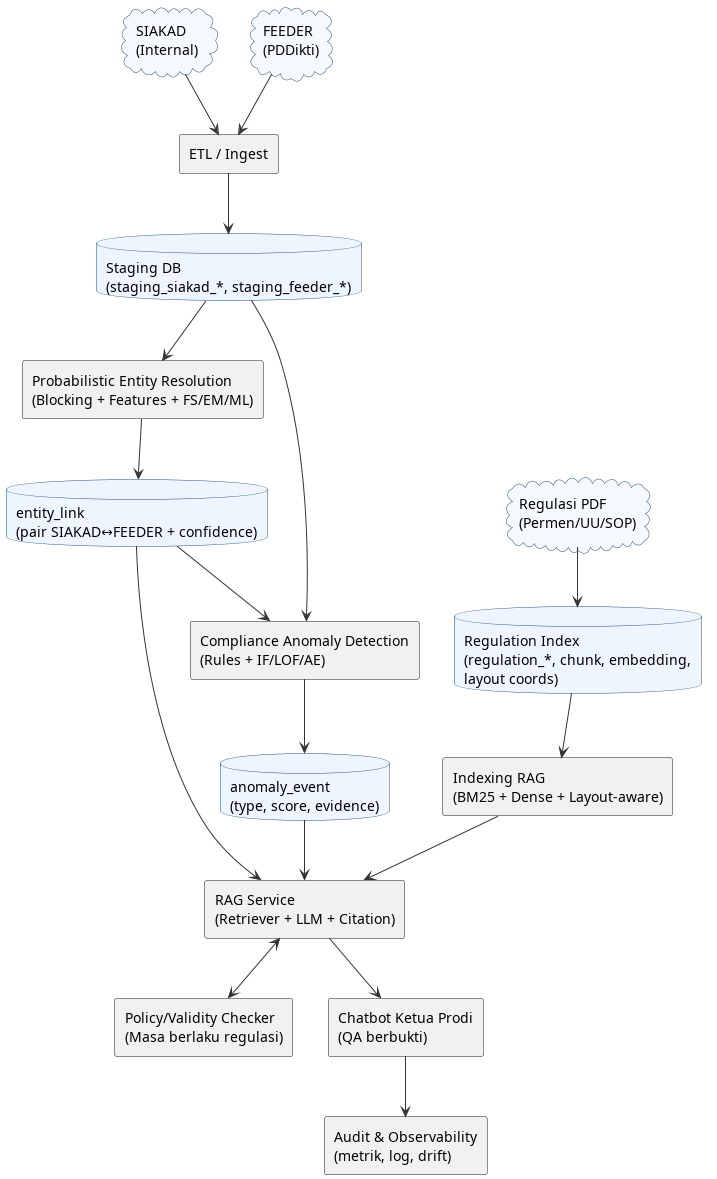
\includegraphics[width=0.7\linewidth]{DiagramKerangkaKonseptual.png}
                \caption{Diagram Kerangka Konseptual}
                \label{fig:kerangka}
            \end{figure}
    % ===================== HALAMAN BAB 4 (spasi 1.5) =====================
    \chapter{METODOLOGI PENELITIAN}
        \thispagestyle{empty}

        \section{Desain Penelitian}
        Penelitian ini dirancang dengan pendekatan \textit{experimental research} berbasis rekayasa perangkat lunak dan analitik data. Fokus utamanya adalah membangun prototipe sistem audit kepatuhan akademik yang mengintegrasikan:
        \begin{enumerate}
            \item \textbf{Data Alignment (Probabilistic Entity Resolution)} antara SIAKAD internal dan FEEDER PDDikti.
            \item \textbf{Compliance Anomaly Detection} berbasis metode hibrida (aturan regulasi + algoritma deteksi outlier).
            \item \textbf{Retrieval-Augmented Generation (RAG)} untuk menjawab pertanyaan pimpinan program studi dengan bukti regulasi dan data hasil alignment.
        \end{enumerate}

        Desain penelitian ini bersifat \textit{design science research}, di mana kontribusi utama berupa model konseptual, algoritme, serta prototipe sistem yang divalidasi melalui uji coba dataset riil dan evaluasi kuantitatif maupun kualitatif.

        \section{Dataset Penelitian}
        Dataset yang digunakan terdiri atas tiga kategori:
        \begin{enumerate}
            \item \textbf{Data Akademik SIAKAD} (read-only) dari universitas studi kasus: mencakup data mahasiswa, dosen, mata kuliah, kelas, dan registrasi.
            \item \textbf{Data FEEDER PDDikti} (read-only) sebagai kanal pelaporan resmi: mencakup entitas sepadan (mahasiswa, dosen, prodi, mata kuliah).
            \item \textbf{Dokumen Regulasi Pendidikan Tinggi}: Permenristekdikti No. 51 dan 52 Tahun 2018, Permendikbudristek No. 50 Tahun 2024, Permendikbudristek No. 53 Tahun 2023, dan regulasi terbaru Permendikbudristek No. 39 Tahun 2025.
        \end{enumerate}

        Untuk menjaga privasi, data mahasiswa/dosen akan dianonimkan. Dataset diproses melalui pipeline ETL ke dalam \texttt{staging\_siakad\_*}, \texttt{staging\_feeder\_*}, serta \texttt{regulation\_*} sebelum dilakukan eksperimen.

        \section{Tahapan Eksperimen}
        Eksperimen penelitian terdiri atas lima tahap utama:
        \begin{enumerate}
            \item \textbf{Preprocessing dan ETL}
            \begin{itemize}
                \item Ekstraksi data SIAKAD–FEEDER ke tabel \texttt{staging}.
                \item Ekstraksi teks regulasi PDF dengan OCR + segmentasi layout (pasal, ayat, tabel).
            \end{itemize}

            \item \textbf{Probabilistic Entity Resolution (ER)}
            \begin{itemize}
                \item Pemodelan pasangan kandidat entitas (blocking berdasarkan kunci: NIM, NIDN, nama).
                \item Penghitungan skor probabilitas kesamaan dengan model Fellegi–Sunter, embedding (BERT/IndoBERT), dan classifier ML (LogReg/GBM).
                \item Output: tabel \texttt{entity\_link} berisi pasangan entitas dan \textit{confidence score}.
            \end{itemize}

            \item \textbf{Deteksi Anomali Kepatuhan}
            \begin{itemize}
                \item Penerapan aturan regulasi eksplisit (misalnya SKS dosen $\leq$ 16, masa studi $\leq$ 7 tahun).
                \item Penerapan algoritme deteksi anomali: Isolation Forest, LOF, dan Autoencoder.
                \item Output: tabel \texttt{anomaly\_event} berisi jenis anomali, skor, dan bukti regulasi.
            \end{itemize}

            \item \textbf{Retrieval-Augmented Generation (RAG)}
            \begin{itemize}
                \item Indeks dokumen regulasi dengan BM25 + dense embedding (FAISS).
                \item Integrasi hasil \texttt{entity\_link} dan \texttt{anomaly\_event} ke retriever.
                \item LLM (misalnya LLaMA 3.1 atau GPT-4) menghasilkan jawaban dengan sitasi bukti.
            \end{itemize}

            \item \textbf{Integrasi Sistem dan Antarmuka Chatbot}
            \begin{itemize}
                \item Pembuatan layanan API \texttt{/ask}, \texttt{/retrieve}, \texttt{/cite}.
                \item Antarmuka chatbot berbasis web untuk ketua program studi.
                \item Logging audit dan observability (monitoring performa, metrik keandalan).
            \end{itemize}
        \end{enumerate}

        \section{Rencana Evaluasi}
        Evaluasi penelitian dilakukan melalui tiga dimensi:
        \begin{enumerate}
            \item \textbf{Evaluasi Entity Resolution}
            \begin{itemize}
                \item Metrik: Precision, Recall, F1-Score.
                \item Baseline: rule-based matching sederhana.
            \end{itemize}

            \item \textbf{Evaluasi Anomaly Detection}
            \begin{itemize}
                \item Metrik: AUC, Precision@k, interpretabilitas hasil.
                \item Validasi: perbandingan dengan catatan manual staf akademik.
            \end{itemize}

            \item \textbf{Evaluasi RAG}
            \begin{itemize}
                \item Faithfulness: QAFactEval, FactScore.
                \item Citation Precision: persentase jawaban yang benar-benar disertai bukti regulasi valid.
                \item Studi pengguna: wawancara dan kuesioner dengan pimpinan program studi untuk menilai kegunaan, akurasi persepsi, dan tingkat kepercayaan.
            \end{itemize}

            \item \textbf{Evaluasi End-to-End}
            \begin{itemize}
                \item Kecepatan respon sistem (latensi end-to-end).
                \item Kepatuhan terhadap Permendikbudristek No. 39 Tahun 2025.
                \item Dampak praktis: potensi pengurangan beban manual staf akademik.
            \end{itemize}
        \end{enumerate}

        \section{Ringkasan}
        Metodologi penelitian ini membentuk alur sistematis: ETL → Entity Resolution → Anomaly Detection → RAG → Evaluasi. Pendekatan ini memastikan kontribusi penelitian tidak hanya pada level algoritmik, tetapi juga pada implementasi nyata sistem audit kepatuhan berbasis AI untuk pendidikan tinggi di Indonesia.

    % ===================== DAFTAR PUSTAKA (spasi 1) =====================
    \printbibliography[title={Daftar Pustaka}]
\end{document}
